% Provenance (never printed): see sources/outline_sources.md (Year 3:
% speciation and saturation indices; carbonate equilibria applied to rocks;
% weathering kinetics; hydrothermal fluids). Brief: sources/book5/BRIEFS.md,
% ch. 15. Curves from figdata/bachelor-3/carbonate_system.py,
% activity_diagram.py, weathering_rates.py. Exercise and problem values in the
% Book 5 scratch calculator calc/ch15.py. The spring below the Varden
% limestone, its analysis and the granite stream are invented.
\chapter{Water--Rock Interaction}\label{ch:b3:water-rock-interaction}

A spring at the foot of a limestone escarpment leaves a white crust on every
twig and stone it touches; a stream draining a granite carries silica, sodium
and a little potassium, and leaves no crust at all. The difference is in the
water's chemistry, and the chemistry is a record of the rock the water
crossed: how much carbon dioxide it carried, how long it stayed, which
minerals it dissolved and which it built. This chapter reads that record with
the tools of solution chemistry, from the analysis of a water to the rates of
mineral dissolution and the isotopic traces of hot fluids in the crust.

\begin{recall}
Activity, activity coefficient, ionic strength, speciation, the solubility
product, alkalinity, the saturation state $\Omega$, Henry's law, rate laws,
the Arrhenius law, the transition state and the $\delta$ value are in the
chemistry books' university volumes. Chemical weathering, the hydrolysis of
silicates, clay minerals and kaolinite are in the Year 1 volume, in its
chapter on weathering and clays; the lysocline and the carbonate compensation
depth in its chapter on carbonate, siliceous and evaporite sediments. The
hydrothermal fluid is in the Year 2 volume, in its chapter on ore deposits,
and the silicate-weathering thermostat in its chapter on climate over
geological time; hydrothermal circulation is in the school books.
\end{recall}

\section{The analysis of a natural water}\label{sec:b3:water-rock-interaction:analysis}

A water analysis lists the major ions in milligrams per litre: calcium,
magnesium, sodium and potassium; bicarbonate, chloride, sulfate and nitrate;
dissolved silica as \ce{SiO2}; and the pH and temperature measured at the
source, since both change once the sample leaves it. Dividing by the molar
mass gives millimoles per litre, and multiplying by the charge,
milliequivalents. A dilute water is electrically neutral, so the sum of the
cations must equal the sum of the anions.

\begin{method}[Checking a water analysis]\label{met:b3:water-rock-interaction:analysis}
\begin{enumerate}
\item convert each concentration to \unit{mmol/L} and to \unit{meq/L};
\item sum the cations and the anions in \unit{meq/L};
\item compute the charge-balance error $100\,(\sum\text{cat} -
  \sum\text{an})/(\sum\text{cat} + \sum\text{an})$, in per cent;
\item accept the analysis if the error is within 1 or \qty{2}{\percent} for a
  water of 250 to \qty{1000}{mg/L}, a little more for a more dilute one;
  otherwise look for a missing ion or an analytical error.
\end{enumerate}
\end{method}
% ledger: hem85:charge-balance

The activity of an ion is its molality times its activity coefficient
$\gamma$. In natural waters $\gamma$ is computed from the ionic strength $I =
\tfrac12\sum m_i z_i^2$ with the extended Debye--Hückel equation
\[
-\log\gamma_i = \frac{A z_i^2\sqrt I}{1 + B a_i\sqrt I},
\]
with $A = 0.5085$ and $B = 0.3281$ for water at \qty{25}{\celsius}, and an
ion size $a_i$ in ångströms: 9 for \ce{H+}, 8 for \ce{Mg^2+}, 6 for
\ce{Ca^2+}, 5 for \ce{CO3^2-}, 4 for \ce{Na+}, \ce{HCO3-} and \ce{SO4^2-},
3 for \ce{K+}, \ce{Cl-}, \ce{OH-} and \ce{NO3-}. The equation is good up to
about \qty{0.1}{mol/L} of univalent salts, which covers rivers and most
ground waters but not seawater or brines. Temperature changes $A$ only from
0.4883 at \qty{0}{\celsius} to 0.5425 at \qty{60}{\celsius}, so the values at
\qty{25}{\celsius} serve for cool waters too.
% ledger: hem85:debye-huckel

The inorganic carbon of a water is shared among dissolved carbon dioxide
(written \ce{CO2} for the sum of \ce{CO2} and \ce{H2CO3}), bicarbonate and
carbonate, linked by
\[
K_1 = \frac{a_{\ce{HCO3-}}\,a_{\ce{H+}}}{a_{\ce{CO2}}}, \qquad
K_2 = \frac{a_{\ce{CO3^2-}}\,a_{\ce{H+}}}{a_{\ce{HCO3-}}}, \qquad
K_H = \frac{a_{\ce{CO2}}}{P_{\ce{CO2}}},
\]
with $\log K_1 = -6.35$, $\log K_2 = -10.33$ and $\log K_H = -1.47$ at
\qty{25}{\celsius}, and $-6.46$, $-10.49$ and $-1.27$ at \qty{10}{\celsius}
($P$ in atmospheres). Between pH 6.4 and 10.3 bicarbonate dominates, and in
most natural waters the alkalinity is nearly all bicarbonate. A measured pH
and bicarbonate then give the other two species, and the partial pressure of
carbon dioxide the water would be in equilibrium with.
% ledger: phreeqc:carbonate

\section{Saturation}\label{sec:b3:water-rock-interaction:saturation}

\begin{definition}[Saturation index]\label{def:b3:water-rock-interaction:si}
The \emph{saturation index (of a mineral)}\index{saturation index (of a mineral)}
in a water is $\mathrm{SI} = \log(\mathrm{IAP}/K)$, where IAP is
the ion activity product of the water written like the mineral's solubility
product $K$: $\mathrm{SI} = \log\Omega$.
\end{definition}

A water with $\mathrm{SI} < 0$ can dissolve the mineral, one with
$\mathrm{SI} > 0$ can precipitate it, and $\mathrm{SI} = 0$ is equilibrium.
Since the free energy of the dissolution reaction is $\Delta_r G = RT\ln\Omega
= 2.303\,RT\,\mathrm{SI}$, the saturation index is also a measure of the
driving force, in units of $2.303\,RT$, about \qty{5.7}{kJ/mol} at
\qty{25}{\celsius}. For calcite $\mathrm{IAP} = a_{\ce{Ca^2+}}
a_{\ce{CO3^2-}}$ and $\log K = -8.45$ at \qty{25}{\celsius}, $-8.35$ at
\qty{10}{\celsius}: calcite is more soluble in cold water. For gypsum, $\mathrm{SI} = \log(a_{\ce{Ca^2+}}a_{\ce{SO4^2-}}) + 4.55$;
for quartz, whose dissolution gives neutral \ce{H4SiO4}, $\mathrm{SI} = \log
a_{\ce{H4SiO4}} + 3.98$, and for amorphous silica the constant is 2.71
instead of 3.98. Measured indices carry an uncertainty of at least $\pm0.1$,
and a water within $\pm0.3$ of zero is taken as close to equilibrium.
% ledger: phreeqc:carbonate, phreeqc:silicates, hem85:si

\section{Carbonate equilibria in rocks}\label{sec:b3:water-rock-interaction:carbonate}

Calcite dissolves in water charged with carbon dioxide by
\[
\ce{CaCO3 + CO2 + H2O <=> Ca^2+ + 2 HCO3-},
\qquad K = \frac{a_{\ce{Ca^2+}}\,a_{\ce{HCO3-}}^2}{P_{\ce{CO2}}}
= \frac{K_{\mathrm{cal}}K_1K_H}{K_2},
\]
with $\log K = -5.94$ at \qty{25}{\celsius} and $-5.59$ at \qty{10}{\celsius}.
How much dissolves depends on where the carbon dioxide comes from.

\begin{definition}[Open and closed carbonate systems]\label{def:b3:water-rock-interaction:open-closed}
A water dissolves calcite in an \emph{open carbonate system}\index{open carbonate system}
when it stays in contact with a gas of fixed
$P_{\ce{CO2}}$, which replaces the carbon dioxide used. It does so in a
\emph{closed carbonate system}\index{closed carbonate system} when it was
charged with carbon dioxide first and then isolated from the gas, so that
the carbon dioxide it holds is all it can use.
\end{definition}

\begin{theorem}[Calcite solubility, open and closed]\label{thm:b3:water-rock-interaction:calcite}
For a water of calcium bicarbonate type, with $m$ the molality of calcium,
\[
\text{open:}\quad m = \left(\frac{K\,P_{\ce{CO2}}}{4\gamma_{\ce{Ca^2+}}
\gamma_{\ce{HCO3-}}^2}\right)^{1/3};
\qquad
\text{closed:}\quad 4\gamma_{\ce{Ca^2+}}\gamma_{\ce{HCO3-}}^2\,m^3 =
\frac{K_{\mathrm{cal}}K_1}{K_2}\,(C_0 - m),
\]
where $C_0 = K_H P_{\ce{CO2}}$ is the carbon dioxide taken up before the
system closed.
\end{theorem}

\begin{proof}
Between pH 6.5 and 8.5 carbonate, \ce{H+} and \ce{OH-} are negligible next to
bicarbonate, so the charge balance is $2m = m_{\ce{HCO3-}}$. Open: $K = \gamma
_{\ce{Ca^2+}}m\,\gamma_{\ce{HCO3-}}^2(2m)^2/P_{\ce{CO2}}$, which gives the
cube root. Closed: each calcium dissolved uses one \ce{CO2}, so $m_{\ce{CO2}}
= C_0 - m$ and $a_{\ce{Ca^2+}}a_{\ce{HCO3-}}^2/a_{\ce{CO2}} = K/K_H =
K_{\mathrm{cal}}K_1/K_2$ gives the cubic.
\end{proof}

In the open system the calcium grows as the cube root of $P_{\ce{CO2}}$; in
the closed system it is capped by $C_0$, and the carbon dioxide left at the
end, hence the final $P_{\ce{CO2}}$, is much lower than at the start. Soil
air holds 10 to 100 times the carbon dioxide of the atmosphere, made by roots
and by the decay of plant matter, and ground waters commonly show
$P_{\ce{CO2}}$ between $10^{-2.5}$ and $10^{-1}$ atmosphere. Water in contact
with calcite and air holds only about \qty{20}{mg/L} of calcium; rain that
reaches a limestone through a soil, still open to the soil gas, can take
four or five times more. Karst is carved by this soil carbon dioxide.
% ledger: hem85:pco2, phreeqc:carbonate

The way back is degassing. A spring that emerges from a limestone carries
the $P_{\ce{CO2}}$ of the soil and the rock, ten to a hundred times that of
the air. In the open it loses carbon dioxide, bicarbonate turns into
carbonate, the pH rises, and the saturation index climbs by more than a unit,
as panel (b) of the figure below shows for the spring of this chapter's
weekend problem.
Calcite precipitates on the stream bed and on mosses and twigs: tufa from
cold springs, travertine from hot ones. Springs that pass through the rock
quickly, in days or weeks, by conduits, commonly reach the surface
undersaturated; those that seep slowly through it for months emerge near
saturation.
% ledger: hem85:pco2, usgsyvo:travertine

\begin{omfigure}
\begin{tikzpicture}
\begin{groupplot}[group style={group size=2 by 1, horizontal sep=1.6cm},
  omrecord, width=0.47\linewidth, height=0.42\linewidth, title style={font=\small},
  tick label style={font=\scriptsize}, label style={font=\small},
  legend style={font=\scriptsize, legend cell align=left}]
\nextgroupplot[title={(a) calcite solubility},
  xlabel={$\log P_{\ce{CO2}}$ (atm)}, ylabel={dissolved calcium (\unit{mmol/L})},
  xmin=-3.5, xmax=-1, ymin=0, ymax=5.5, clip=false,
  xtick={-3.5,-3,-2.5,-2,-1.5,-1}, xticklabels={$-3.5$,$-3$,$-2.5$,$-2$,$-1.5$,$-1$},
  legend style={at={(0.14,0.97)}, anchor=north west}]
\addplot[draw=none, fill=black!6, forget plot] coordinates {(-2.5,0) (-2.5,5.5) (-1,5.5) (-1,0)} -- cycle;
% computed in figdata/bachelor-3/carbonate_system.py
\addplot[omDef, thick] table[x=logp, y=ca_open10] {figdata/out/bachelor-3-carbonate_system-solubility.dat};
\addlegendentry{open, \qty{10}{\celsius}}
\addplot[red!70!black, thick] table[x=logp, y=ca_open25] {figdata/out/bachelor-3-carbonate_system-solubility.dat};
\addlegendentry{open, \qty{25}{\celsius}}
\addplot[omDef, thick, densely dashed] table[x=logp, y=ca_closed10] {figdata/out/bachelor-3-carbonate_system-solubility.dat};
\addlegendentry{closed, \qty{10}{\celsius}}
\addplot[red!70!black, thick, densely dashed] table[x=logp, y=ca_closed25] {figdata/out/bachelor-3-carbonate_system-solubility.dat};
\addlegendentry{closed, \qty{25}{\celsius}}
\draw[black, densely dotted] (axis cs:-3.37,0) -- (axis cs:-3.37,5.5);
\node[font=\scriptsize, anchor=south] at (axis cs:-3.37,5.5) {air};
\node[font=\scriptsize, anchor=north] at (axis cs:-1.4,5.45) {ground waters};
\nextgroupplot[title={(b) the spring degassing},
  xlabel={$\log P_{\ce{CO2}}$ (atm)}, ylabel={SI of calcite},
  xmin=-3.5, xmax=-1.5, ymin=-0.2, ymax=1.9, x dir=reverse, clip=false,
  xtick={-3.5,-3,-2.5,-2,-1.5}, xticklabels={$-3.5$,$-3$,$-2.5$,$-2$,$-1.5$}]
% computed in figdata/bachelor-3/carbonate_system.py
\addplot[omDef, thick] table[x=logp, y=si] {figdata/out/bachelor-3-carbonate_system-degassing.dat};
\addplot[black, densely dotted, domain=-3.5:-1.5, samples=2] {0};
\addplot[red!70!black, only marks, mark=*, mark size=1.6pt] table[x=logp, y=si] {figdata/out/bachelor-3-carbonate_system-ends.dat};
\node[font=\scriptsize, anchor=north west] at (axis cs:-1.84,-0.01) {outlet};
\node[font=\scriptsize, anchor=north west] at (axis cs:-3.3,1.55) {air};
\end{groupplot}
\end{tikzpicture}

\par\smallskip{\small (a) Calcium dissolved by water in equilibrium with
calcite, against the partial pressure of carbon dioxide (for the closed
system, the pressure the water was charged at): open system solid, closed
system dashed; cold water dissolves more; the grey band is the range of
ground waters. (b) The spring below the Varden limestone, at \qty{10}{\celsius},
losing carbon dioxide on its way down the hill (read from left to right, on a reversed axis)
before any calcite forms: its calcium and alkalinity are fixed, its pH rises
from 7.2 to 8.8, and its saturation index from 0.04 to 1.6. Equilibrium
constants from a public database, extended Debye--Hückel activity
coefficients.}\label{fig:b3:water-rock-interaction:calcite}
\end{omfigure}
% ledger: phreeqc:carbonate, hem85:debye-huckel, hem85:pco2, data:co2-mlo

The same chemistry, run at the scale of the ocean, is in the chemistry
books' university volumes; the depth at which seawater becomes undersaturated
with calcite, the lysocline, and the depth below which calcite does not
accumulate are in the Year 1 volume.

\begin{inthefield}[A spring that builds its own terraces]
\begin{minipage}[t]{0.52\linewidth}\vspace{0pt}
At Palette Spring, one of the Mammoth Hot Springs of the Yellowstone
plateau, thermal water rises through a buried limestone and carries it away
dissolved. At the surface the water
spreads over its own deposits and loses carbon dioxide, and calcium carbonate
precipitates as travertine, on the rim of each pool first, where the water is
thinnest. Geologists who survey these springs measure deposition of about
three millimetres a day, fifteen times the rate of the tufas of cold
springs. The orange and
brown stripes are mats of heat-loving microbes living in the warm runoff.
\end{minipage}\hfill
\begin{minipage}[t]{0.44\linewidth}\vspace{0pt}
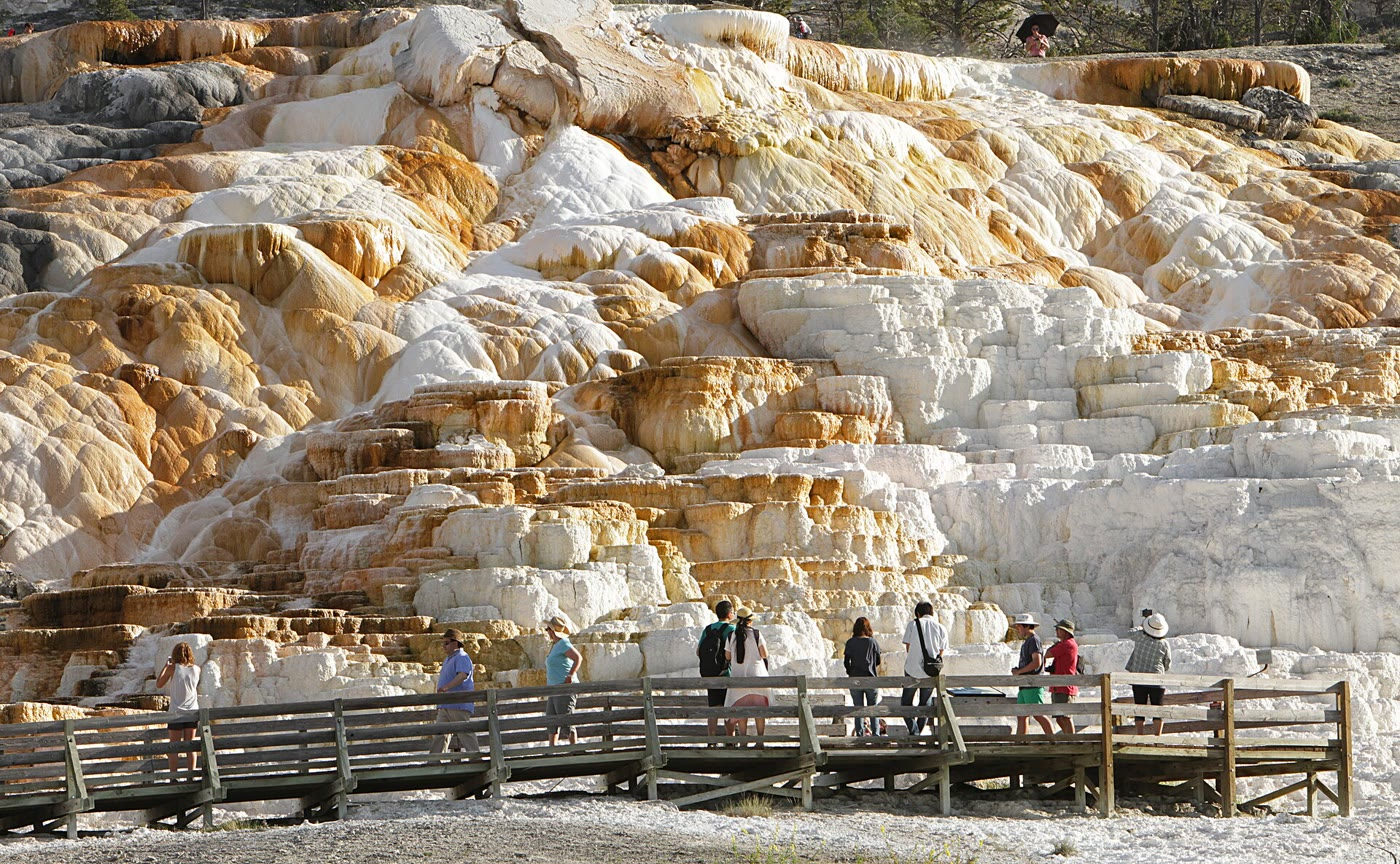
\includegraphics[width=\linewidth]{images/book5/b3-palette-spring-travertine.jpg}

{\scriptsize Travertine terraces of Palette Spring, Mammoth Hot Springs, with
a boardwalk and visitors for scale. NPS photo by Jim Peaco, public domain.}
\end{minipage}
\end{inthefield}
% ledger: photo:b3-palette-spring, usgsyvo:travertine, nps:travertine-terraces

\section{Silicate weathering kinetics}\label{sec:b3:water-rock-interaction:kinetics}

Silicates dissolve far more slowly than calcite, and a water seldom reaches
equilibrium with them: their dissolution has to be described by a rate.

\begin{definition}[Mineral dissolution rate law]\label{def:b3:water-rock-interaction:rate-law}
The \emph{mineral dissolution rate law}\index{mineral dissolution rate law}
gives the rate of dissolution per unit of mineral surface, in
\unit{mol.m^{-2}.s^{-1}}, as a sum over acid, neutral and basic mechanisms,
\[
r = \sum_j k_j\,e^{-\frac{E_j}{R}\left(\frac1T - \frac1{298.15}\right)}\,
a_{\ce{H+}}^{n_j}\,\bigl(1 - \Omega^{p_j}\bigr)^{q_j},
\]
with rate constants $k_j$ at \qty{25}{\celsius}, activation energies $E_j$,
reaction orders $n_j$ (negative for the basic mechanism) and two exponents
$p_j$, $q_j$, commonly taken as 1.
\end{definition}
% ledger: pk04:rate-law

\begin{proposition}[Far from and near equilibrium]\label{prop:b3:water-rock-interaction:affinity}
With $p = q = 1$, the rate does not depend on the saturation of the water
when $\Omega \ll 1$, and near equilibrium it is proportional to the
saturation index: $r \approx -2.303\,r_\infty\,\mathrm{SI}$, where
$r_\infty$ is the rate far from equilibrium.
\end{proposition}

\begin{proof}
The factor is $1 - \Omega = 1 - 10^{\mathrm{SI}}$. For $\mathrm{SI} \ll 0$ it
tends to 1; for $\mathrm{SI}$ near 0, $10^{\mathrm{SI}} \approx 1 +
2.303\,\mathrm{SI}$.
\end{proof}

The rate constants come from laboratory experiments on fresh mineral powders,
in flow-through reactors kept far from equilibrium. The figure below draws
the rate law for four minerals at \qty{25}{\celsius}. Each curve is a V or a
U: protons speed dissolution in acid water, hydroxide in basic water, and in
between the neutral mechanism sets a floor. Olivine dissolves about three
orders of magnitude faster than albite at pH 5, which is why it is the first
of the common silicates to disappear from a soil. The activation energies of
albite and forsterite, 65 to \qty{79}{kJ/mol}, make their rates four to five
times faster at \qty{25}{\celsius} than at \qty{10}{\celsius}.
% ledger: pk04:rates

Field rates are lower, by orders of magnitude. In column experiments on a
freshly crushed granite, the rate of plagioclase fell steadily over six years
to \qty{7.0e-14}{mol.m^{-2}.s^{-1}}; the same granite, naturally weathered
and partly turned to kaolinite, dissolved at \qty{2.1e-15}{mol.m^{-2}.s^{-1}}
under the same conditions, and both are still far faster than the rate
measured in the weathering profile itself. Over many minerals and ages, the
rate falls with the time $t$ the mineral has been weathering as $R =
\num{3.1e-13}\,t^{-0.61}$ (mol\,m$^{-2}$\,s$^{-1}$, $t$ in years). Part of
the decline is in the mineral, whose most reactive surfaces dissolve first;
the rest is in the setting: slow water, much mineral for little fluid, and
pore waters close to equilibrium, where the proposition above makes the rate
small.
% ledger: whitebrantley03:rates

\begin{omfigure}
\begin{tikzpicture}
\begin{axis}[omrecord, width=0.74\linewidth, height=0.46\linewidth,
  xlabel={pH}, ylabel={$\log r$ (\unit{mol.m^{-2}.s^{-1}})},
  xmin=0, xmax=14, ymin=-14.5, ymax=-6, clip=false,
  xtick={0,2,4,6,8,10,12,14}, ytick={-14,-12,-10,-8,-6},
  yticklabels={$-14$,$-12$,$-10$,$-8$,$-6$},
  tick label style={font=\scriptsize}, label style={font=\small},
  legend style={font=\scriptsize, legend cell align=left, at={(1.03,0.5)}, anchor=west}]
% computed in figdata/bachelor-3/weathering_rates.py
\addplot[green!45!black, thick] table[x=ph, y=forsterite] {figdata/out/bachelor-3-weathering_rates-curves.dat};
\addlegendentry{forsterite}
\addplot[omDef, thick] table[x=ph, y=albite] {figdata/out/bachelor-3-weathering_rates-curves.dat};
\addlegendentry{albite}
\addplot[red!70!black, thick, densely dashed] table[x=ph, y=kfeldspar] {figdata/out/bachelor-3-weathering_rates-curves.dat};
\addlegendentry{K-feldspar}
\addplot[black, thick, densely dotted] table[x=ph, y=kaolinite] {figdata/out/bachelor-3-weathering_rates-curves.dat};
\addlegendentry{kaolinite}
\end{axis}
\end{tikzpicture}

\par\smallskip{\small Dissolution rates far from equilibrium at
\qty{25}{\celsius}, against pH, from a published compilation of laboratory
rate parameters. The olivine end-member forsterite has no basic mechanism in
the compilation; its curve stops falling at the neutral floor.}\label{fig:b3:water-rock-interaction:rates}
\end{omfigure}
% ledger: pk04:rates

\begin{definition}[Weathering regimes]\label{def:b3:water-rock-interaction:regimes}
Chemical weathering in a landscape is in a \emph{supply-limited
regime}\index{supply-limited regime} when it is limited by the rate at which
erosion brings fresh minerals to the weathering front, and in a
\emph{weathering-limited regime}\index{weathering-limited regime} when fresh
minerals are abundant and the rate of the reactions limits it.
\end{definition}

A compilation of small catchments shows both. Where erosion is slow, under
thick and leached soils on gentle relief, the weathering flux follows the
erosion rate: whatever fresh rock arrives is fully leached, and a warmer or
wetter climate changes little. Where erosion is fast, in steep mountains, the
flux grows with runoff, as the square root of the erosion rate, and with
temperature, with an apparent activation energy of $74 \pm
\qty{29}{kJ/mol}$. Only in the second regime can silicate weathering act as
the climate thermostat of the Year 2 volume.
% ledger: west05:regimes

Which secondary mineral a weathering water forms is read on another
diagram.

\begin{definition}[Activity diagram]\label{def:b3:water-rock-interaction:activity-diagram}
An \emph{activity diagram (mineral stability)}\index{activity diagram (mineral stability)}
divides a plane of activity ratios of a water, such as
$\log(a_{\ce{K+}}/a_{\ce{H+}})$ against $\log a_{\ce{H4SiO4}}$, into the
fields where each mineral of a chemical system is the stable one.
\end{definition}

\begin{proposition}[Boundaries of an activity diagram]\label{prop:b3:water-rock-interaction:boundaries}
In the system \ce{K2O}--\ce{Al2O3}--\ce{SiO2}--\ce{H2O}, with aluminium conserved in the solids
and water at unit activity, a mineral with $k$ potassium, $a$ aluminium and
$s$ silicon atoms per formula and dissolution constant $K$ (to \ce{K+},
\ce{Al^3+}, \ce{H4SiO4}) fixes
\[
\log\frac{a_{\ce{Al^3+}}}{a_{\ce{H+}}^3} = \frac{\log K - kX - sY}{a},
\qquad X = \log\frac{a_{\ce{K+}}}{a_{\ce{H+}}},\quad Y = \log a_{\ce{H4SiO4}}.
\]
The stable mineral gives the lowest aluminium activity, and the boundary
between two minerals is a straight line in $(Y, X)$.
\end{proposition}

\begin{proof}
The dissolution consumes $h = k + 3a$ protons, by charge balance, so $a\log
a_{\ce{Al^3+}} = \log K + h\log a_{\ce{H+}} - k\log a_{\ce{K+}} - s\log
a_{\ce{H4SiO4}}$; dividing by $a$ and moving $3\log a_{\ce{H+}}$ to the left
gives the expression. A water in equilibrium with one mineral is
undersaturated with any mineral that would need more aluminium, and
supersaturated with any that would need less, so the least soluble one is
stable. Equating two such expressions, linear in $X$ and $Y$, gives a line.
\end{proof}

With the constants at \qty{25}{\celsius}, gibbsite gives way to kaolinite at
$\log a_{\ce{H4SiO4}} = -4.39$ (\qty{2.4}{mg/L} of silica) and kaolinite to
muscovite at $\log(a_{\ce{K+}}/a_{\ce{H+}}) = 1.55$, and K-feldspar is stable
only in waters rich in potassium and silica. The diagram is the weathering
sequence of the Year 1 volume in numbers: a dilute water that flushes
potassium and silica away strips a feldspar down to gibbsite; a water that
keeps more silica makes kaolinite; one that keeps more potassium, as at depth,
makes a mica.
% ledger: phreeqc:silicates

\begin{omfigure}
\begin{tikzpicture}
\begin{axis}[omrecord, width=0.66\linewidth, height=0.5\linewidth,
  xlabel={$\log a_{\ce{H4SiO4}}$}, ylabel={$\log(a_{\ce{K+}}/a_{\ce{H+}})$},
  xmin=-6, xmax=-2, ymin=0, ymax=10, clip=false,
  xtick={-6,-5,-4,-3,-2}, xticklabels={$-6$,$-5$,$-4$,$-3$,$-2$},
  tick label style={font=\scriptsize}, label style={font=\small}]
% computed in figdata/bachelor-3/activity_diagram.py
\addplot[black, thick, unbounded coords=jump] table[x=y, y=x] {figdata/out/bachelor-3-activity_diagram-lines.dat};
\addplot[omDef, densely dashed] table[x=y, y=x] {figdata/out/bachelor-3-activity_diagram-quartz.dat};
\addplot[omDef, densely dotted] table[x=y, y=x] {figdata/out/bachelor-3-activity_diagram-amorph.dat};
\addplot[red!70!black, only marks, mark=*, mark size=1.8pt] table[x=y, y=x] {figdata/out/bachelor-3-activity_diagram-samples.dat};
\node[font=\small] at (axis cs:-5.4,0.8) {gibbsite};
\node[font=\small] at (axis cs:-3.25,0.75) {kaolinite};
\node[font=\small] at (axis cs:-4.6,5.0) {muscovite};
\node[font=\small] at (axis cs:-3.3,9.3) {K-feldspar};
\node[font=\scriptsize, omDef, anchor=south] at (axis cs:-3.98,10) {quartz};
\node[font=\scriptsize, omDef, anchor=south] at (axis cs:-2.71,10) {amorphous silica};
\node[font=\scriptsize, red!70!black, anchor=west] at (axis cs:-4.58,0.38) {A};
\node[font=\scriptsize, red!70!black, anchor=west] at (axis cs:-3.80,1.29) {B};
\node[font=\scriptsize, red!70!black, anchor=west] at (axis cs:-3.48,4.08) {C};
\end{axis}
\end{tikzpicture}

\par\smallskip{\small Stability fields in the system
\ce{K2O}--\ce{Al2O3}--\ce{SiO2}--\ce{H2O} at \qty{25}{\celsius}, with the saturation of quartz
(dashed) and amorphous silica (dotted). Three invented waters: A, a dilute
tropical stream; B, a stream on granite; C, a deep ground water in
granite.}\label{fig:b3:water-rock-interaction:activity}
\end{omfigure}
% ledger: phreeqc:silicates

\section{Hydrothermal fluids}\label{sec:b3:water-rock-interaction:hydrothermal}

Hot water circulating through the crust, near a ridge or an intrusion,
exchanges oxygen with the rock it crosses. At high temperature the
fractionation between rock and water is small, and both move toward
isotopic equilibrium: meteoric water, light, makes the rock lighter, and the
water heavier. How far the rock has moved measures how much water has
passed.

\begin{definition}[Water--rock ratio]\label{def:b3:water-rock-interaction:water-rock-ratio}
The \emph{water--rock ratio}\index{water--rock ratio} $W/R$ of a
hydrothermal system is the mass of water that has exchanged with a mass of
rock, divided by that mass of rock.
\end{definition}

\begin{proposition}[Water--rock ratios from oxygen isotopes]\label{prop:b3:water-rock-interaction:wr}
Let a rock of initial $\delta_r^i$ exchange oxygen with a water of initial
$\delta_w^i$ until it reaches $\delta_r^f$, in equilibrium with the water
it last met, $\Delta = \delta_r^f - \delta_w^f$, and let $c_r$ and $c_w$ be
the oxygen concentrations of rock and water. In a closed system (one batch of
water) and in an open one (water passing once),
\[
\frac WR\Big|_{\text{closed}} = \frac{c_r}{c_w}\,
\frac{\delta_r^f - \delta_r^i}{\delta_w^i - \delta_r^f + \Delta},
\qquad
\frac WR\Big|_{\text{open}} = \frac{c_r}{c_w}\,
\ln\!\left(\frac{\delta_r^f - \delta_r^i}{\delta_w^i - \delta_r^f + \Delta} + 1\right).
\]
\end{proposition}

\begin{proof}
Closed: oxygen-18 is conserved, $c_wW\delta_w^i + c_rR\delta_r^i = c_wW
\delta_w^f + c_rR\delta_r^f$, with $\delta_w^f = \delta_r^f - \Delta$; solve
for $W/R$. Open: a parcel $\mathrm dW$ enters at $\delta_w^i$ and leaves in
equilibrium with the rock, at $\delta_r - \Delta$, so $c_rR\,\mathrm d\delta_r
= c_w(\delta_w^i - \delta_r + \Delta)\,\mathrm dW$. Separating,
$\int_{\delta_r^i}^{\delta_r^f}\mathrm d\delta_r/(\delta_w^i - \delta_r +
\Delta) = (c_w/c_r)\,W/R$, and the integral is $-\ln[(\delta_w^i - \delta_r^f
+ \Delta)/(\delta_w^i - \delta_r^i + \Delta)]$, which is the expression.
\end{proof}

For oxygen $c_r/c_w$ is close to 0.5. The open system always needs less
water than the closed one for the same shift, because every parcel leaves
as heavy as it can. Around many intrusions the $\delta^{18}\mathrm O$ of the
country rock draws a bull's-eye of low values, from about $+6$ down to below
0, centred where the most water passed; the ores of the hydrothermal fluid
are often inside the lowest contour, which makes the map an exploration
tool.
% ledger: white13c9:water-rock

\begin{omfigure}
\begin{tikzpicture}[font=\small, >=Stealth]
\draw[thick, fill=black!6] (0,0) rectangle (4,2.2);
\node at (2,1.55) {rock, mass $R$};
\node at (2,0.95) {$\delta_r^i \to \delta_r^f$};
\node[font=\scriptsize] at (2,0.4) {exchange at temperature $T$};
\draw[->, thick, omDef] (-2.6,1.1) -- (-0.1,1.1);
\node[omDef, anchor=south, align=center, font=\scriptsize] at (-1.35,1.15) {water in\\ $\delta_w^i$, $\mathrm dW$};
\draw[->, thick, red!70!black] (4.1,1.1) -- (6.6,1.1);
\node[red!70!black, anchor=south, align=center, font=\scriptsize] at (5.35,1.15) {water out\\ $\delta_r - \Delta$};
\node[anchor=north, font=\scriptsize, align=center] at (2,-0.15) {open system: each parcel passes once and leaves in\\ equilibrium with the rock it last met};
\end{tikzpicture}

\par\smallskip{\small The box model of a hydrothermal system. In a closed
system one batch of water stays with the rock until both are in equilibrium;
in an open system water flows through, and the rock moves toward the water a
little with every parcel.}\label{fig:b3:water-rock-interaction:box}
\end{omfigure}

\begin{definition}[Reaction-path model]\label{def:b3:water-rock-interaction:reaction-path}
A \emph{reaction-path model}\index{reaction-path model} follows the
composition of a water and the minerals it forms as a reaction progresses,
by adding small amounts of a reactant (a mineral dissolving, a gas leaving,
heat removed) and recomputing the speciation and the saturation indices at
each step, precipitating any mineral that reaches saturation.
\end{definition}

A \omterm{def:b3:water-rock-interaction:reaction-path}{reaction-path model} run on the spring of the weekend problem, degassing
step by step, precipitates calcite as soon as its index exceeds zero; run on
a granite and a rain water, it makes gibbsite first, then kaolinite, then
mica as the water collects silica and potassium, tracing a path across the
activity diagram. Speciation programs do this with databases of equilibrium
constants such as the ones used in this chapter.
% ledger: phreeqc:silicates

\section{Exercises}

\begin{exercise}[$\star$]\label{exo:b3:water-rock-interaction:1}
A water has (in \unit{mg/L}) \ce{Ca} 48, \ce{Mg} 9.7, \ce{Na} 23, \ce{K} 3.9,
\ce{HCO3} 183, \ce{Cl} 35.5 and \ce{SO4} 48. Compute its charge-balance
error. Is the analysis acceptable?
\end{exercise}

\begin{exercise}[$\star$]\label{exo:b3:water-rock-interaction:2}
At an ionic strength of 0.0050, compute the activity coefficients of
\ce{Ca^2+}, \ce{HCO3-} and \ce{SO4^2-}.
\end{exercise}

\begin{exercise}[$\star$]\label{exo:b3:water-rock-interaction:3}
A water draining a gypsum-bearing marl holds \qty{3.0}{mmol/L} of calcium and
\qty{4.0}{mmol/L} of sulfate, at an ionic strength of 0.016. Compute the
saturation index of gypsum. Can the water still dissolve gypsum?
\end{exercise}

\begin{exercise}[$\star$]\label{exo:b3:water-rock-interaction:4}
A ground water holds \qty{12}{mg/L} of silica, reported as \ce{SiO2} and
present as \ce{H4SiO4}. Compute its saturation indices for quartz and for
amorphous silica at \qty{25}{\celsius}.
\end{exercise}
% ledger: phreeqc:silicates

\begin{exercise}[$\star\star$]\label{exo:b3:water-rock-interaction:5}
With activity coefficients taken as 1, compute the calcium dissolved by an
open system at $P_{\ce{CO2}} = 10^{-2}$~atm at \qty{25}{\celsius} and at
\qty{10}{\celsius}, in \unit{mmol/L} and \unit{mg/L}.
\end{exercise}

\begin{exercise}[$\star\star$]\label{exo:b3:water-rock-interaction:6}
A water at \qty{25}{\celsius} has pH 7.60 and \qty{4.0}{mmol/L} of
bicarbonate. With activity coefficients of 1, compute its dissolved carbon
dioxide and carbonate, its $P_{\ce{CO2}}$ and the share of each species in
the dissolved inorganic carbon.
\end{exercise}

\begin{exercise}[$\star\star$]\label{exo:b3:water-rock-interaction:7}
An albite grain is a sphere \qty{1}{mm} across in a soil water of pH 5 at
\qty{25}{\celsius}, dissolving at the rate of the figure, $\log r = -12.09$.
With a molar volume of \qty{101.31}{cm^3/mol}, how fast does its radius
shrink, and how long does it last?
\end{exercise}
% ledger: pk04:rates, phreeqc:silicates

\begin{exercise}[$\star\star$]\label{exo:b3:water-rock-interaction:8}
By what factor does the neutral dissolution rate of albite ($E =
\qty{69.8}{kJ/mol}$) grow from \qty{5}{\celsius} to \qty{25}{\celsius}? And
a weathering flux with $E = \qty{74}{kJ/mol}$?
\end{exercise}
% ledger: pk04:rates, west05:regimes

\begin{exercise}[$\star\star$]\label{exo:b3:water-rock-interaction:9}
Derive the kaolinite--muscovite boundary of the activity diagram from the
constants $\log K = 7.435$ (kaolinite, 2 Al, 2 Si) and $12.703$ (muscovite, 1
K, 3 Al, 3 Si). A water at \qty{25}{\celsius} has \qty{2.0}{mg/L} of
potassium, \qty{15}{mg/L} of silica and pH 7.0: which mineral does it form?
\end{exercise}
% ledger: phreeqc:silicates

\begin{exercise}[$\star\star\star$]\label{exo:b3:water-rock-interaction:10}
Near an intrusion, a granodiorite of $\delta^{18}\mathrm O = +6$ is found
at $-2$ (\unit{\permil}). The meteoric water had $-13$, and at the
temperature of exchange the rock was \qty{2}{\permil} heavier than the
water. With $c_r/c_w = 0.5$, compute the \omterm{def:b3:water-rock-interaction:water-rock-ratio}{water--rock ratio} for a closed and
an open system, and explain why they differ.
\end{exercise}
% ledger: white13c9:water-rock

\begin{exercise}[$\star\star\star$]\label{exo:b3:water-rock-interaction:11}
Rain charged with soil gas at $P_{\ce{CO2}} = 10^{-1.5}$~atm at
\qty{10}{\celsius} reaches a limestone. With activity coefficients of 1,
compute the calcium it dissolves if it stays open to the soil gas and if it
is first isolated from it. What fraction of its carbon dioxide is left in the
closed case, and what is its final $P_{\ce{CO2}}$?
\end{exercise}

\begin{exercise}[$\star\star\star$]\label{exo:b3:water-rock-interaction:12}
Using the proposition on rates near equilibrium, what fraction of its
far-from-equilibrium rate does a mineral dissolve at with $\mathrm{SI} =
-2$, $-1$ and $-0.1$? A laboratory rate measured after 6 years of reaction
follows the power law of the chapter: by what factor will it have fallen
after \num{10000} years? Combine both effects to explain why field rates are
so low.
\end{exercise}
% ledger: whitebrantley03:rates

\section{Problem: The Spring below the Varden Limestone}

\begin{problem}[{Weekend problem --- the analysis, carbon dioxide and
saturation of an invented limestone spring, and a granite stream}]
\label{pb:b3:water-rock-interaction:1}
A spring rises at the foot of the Jurassic limestone of the Varden Hills, at
\qty{10}{\celsius} and pH 7.20. Its analysis is (in \unit{mg/L}): \ce{Ca}
112, \ce{Mg} 4.0, \ce{Na} 7.0, \ce{K} 1.2, \ce{HCO3} 340, \ce{Cl} 11,
\ce{SO4} 14, \ce{NO3} 9. At \qty{10}{\celsius}: $\log K_{\mathrm{cal}} =
-8.35$, $\log K_1 = -6.46$, $\log K_2 = -10.49$, $\log K_H = -1.27$. Use the
extended Debye--Hückel equation of the chapter, ignore ion pairs, and take
the air at $\log P_{\ce{CO2}} = -3.37$.

\medskip\noindent\textbf{Part I --- The analysis.}
\begin{enumerate}
\item Convert the analysis to \unit{mmol/L}.
\item Compute the charge-balance error. Is the analysis acceptable?
\item Compute the ionic strength.
\item Compute the activity coefficients of \ce{Ca^2+}, \ce{HCO3-} and
  \ce{CO3^2-}.
\item Is the extended Debye--Hückel equation valid here?
\end{enumerate}

\medskip\noindent\textbf{Part II --- Carbon dioxide.}
\begin{enumerate}[resume]
\item Compute the activity of bicarbonate.
\item Compute the activity of dissolved carbon dioxide.
\item Compute the $P_{\ce{CO2}}$ of the spring. How many times that of the
  air is it, and where can the carbon dioxide come from?
\item Compute the carbonate concentration and the share of each species in
  the dissolved inorganic carbon.
\item Check that the alkalinity is nearly all bicarbonate.
\end{enumerate}

\medskip\noindent\textbf{Part III --- Saturation and travertine.}
\begin{enumerate}[resume]
\item Compute the ion activity product and the saturation index of calcite
  at the outlet.
\item Is the spring in equilibrium with calcite? Is it a conduit spring or
  a slow, diffuse one?
\item Compute the calcium of an open system in equilibrium with calcite at
  the spring's $P_{\ce{CO2}}$, with the activity coefficients of question 4,
  and compare with the analysis.
\item The water degasses to the air before any calcite forms. Keeping the
  bicarbonate activity unchanged, compute its pH and its saturation index.
\item Estimate the calcium it keeps once it has precipitated calcite back to
  equilibrium with the air (open system, activity coefficients at the new
  ionic strength $3m$), and the mass of calcite per litre.
\item The spring flows at \qty{2.0}{L/s} and spreads its deposit over
  \qty{400}{m^2}. If all that calcite stayed there, at a density of
  \qty{2.71}{g/cm^3}, how fast would the deposit grow?
\end{enumerate}

\medskip\noindent\textbf{Part IV --- The granite stream.} A stream on the
Varden granite, under a thick soil on gentle slopes, has (at
\qty{25}{\celsius}) \qty{1.2}{mg/L} of potassium, \qty{9.0}{mg/L} of
silica and pH 5.8.
\begin{enumerate}[resume]
\item Compute its position on the activity diagram.
\item Which mineral does it form? Compute its saturation index for quartz.
\item Below what silica concentration would it make gibbsite?
\item At what pH would it reach the kaolinite--muscovite boundary?
\item Compute the dissolution rate of K-feldspar in this water, far from
  equilibrium, from the parameters $\log k = -10.06$, $n = 0.500$ (acid);
  $-12.41$ (neutral); $-21.20$, $n = -0.823$ (basic).
\item Is the weathering of this catchment more likely supply-limited or
  weathering-limited? Why?
\item With an apparent activation energy of \qty{74}{kJ/mol}, by what factor
  would a weathering-limited flux change between \qty{10}{\celsius} and
  \qty{25}{\celsius}?
\item State the saturation index of calcite of the spring water at its
  outlet.
\end{enumerate}
\end{problem}
% ledger: phreeqc:carbonate, phreeqc:silicates, hem85:debye-huckel, hem85:charge-balance, hem85:si, hem85:pco2, pk04:rates, west05:regimes, data:co2-mlo
